\documentclass[border=5pt]{standalone}
\usepackage[UTF8]{ctex}
\usepackage{amsmath}
\usepackage{tikz}
\usetikzlibrary{positioning, arrows.meta, calc}

\begin{document}
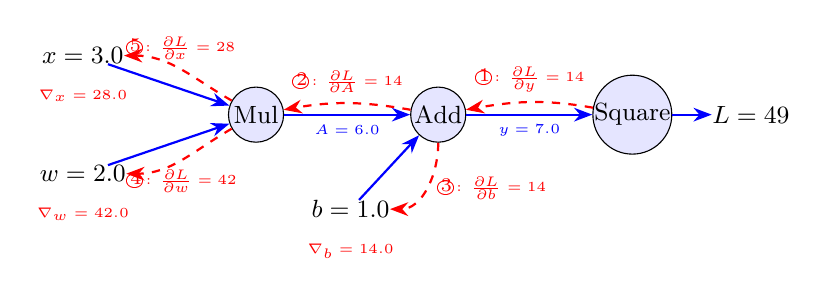
\begin{tikzpicture}[
    node distance=1.2cm,
    every node/.style={align=center},
    op/.style={circle, draw, minimum size=0.7cm, inner sep=0pt, fill=blue!10, font=\small},
    input/.style={inner sep=0pt, font=\small},
    fwdarrow/.style={-Stealth, thick, blue},
    bkarrow/.style={-Stealth, thick, red, dashed},
    label/.style={font=\tiny}
]

% 输入节点
\node[input] (x) at (-3, 0.75) {$x = 3.0$};
\node[input] (w) at (-3, -0.75) {$w = 2.0$};
\node[input] (b) at (0.4, -1.2) {$b = 1.0$};

% 操作节点
\node[op] (mul) at (-0.8, 0) {Mul};
\node[op, right=1.6cm of mul] (add) {Add};
\node[op, right=1.6cm of add] (square) {Square};
\node[input, right=0.5cm of square] (loss) {$L = 49$};

% 前向传播
\draw[fwdarrow] (x) -- (mul);
\draw[fwdarrow] (w) -- (mul);
\draw[fwdarrow] (mul) -- node[below, label] {$A = 6.0$} (add);
\draw[fwdarrow] (b) -- (add);
\draw[fwdarrow] (add) -- node[below, label] {$y = 7.0$} (square);
\draw[fwdarrow] (square) -- (loss);

% 反向传播
% ①: ∂L/∂y
\draw[bkarrow] (square) to[out=170,in=10] node[above, label] {\textcircled{\scriptsize 1}: $\frac{\partial L}{\partial y} = 14$} (add);

% ②: ∂L/∂A
\draw[bkarrow] (add) to[out=170,in=10] node[above, label] {\textcircled{\scriptsize 2}: $\frac{\partial L}{\partial A} = 14$} (mul);

% ③: ∂L/∂b
\draw[bkarrow] (add) to[out=-90,in=0] node[right, label] {\textcircled{\scriptsize 3}: $\frac{\partial L}{\partial b} = 14$} (b);

% ④: ∂L/∂w
\draw[bkarrow] (mul) to[out=-150,in=0] node[below, label] {\textcircled{\scriptsize 4}: $\frac{\partial L}{\partial w} = 42$} (w);

% ⑤: ∂L/∂x
\draw[bkarrow] (mul) to[out=150,in=0] node[above, label] {\textcircled{\scriptsize 5}: $\frac{\partial L}{\partial x} = 28$} (x);

% 梯度值标注
\node[below=0.2cm of x, color=red, font=\tiny] {$\nabla_x = 28.0$};
\node[below=0.2cm of w, color=red, font=\tiny] {$\nabla_w = 42.0$};
\node[below=0.2cm of b, color=red, font=\tiny] {$\nabla_b = 14.0$};

\end{tikzpicture}
\end{document} 
